\documentclass[journal]{IEEEtran}
\usepackage[a5paper, margin=10mm, onecolumn]{geometry}
\usepackage[cmex10]{amsmath}
\usepackage{amssymb,amsfonts,amsthm}
\usepackage{gvv-book}
\usepackage{gvv}
\usepackage{hyperref}
\usepackage{physics}

\begin{document}
\title{4.7.11}
\author{EE25BTECH11025 - Ganachari Vishwambhar}
\maketitle

\textbf{Question}:\\
Show that the path of a moving point such that its distance from two lines  $3x-2y=5$ and $3x+2y=5$ are equal is a straight line.\\
\textbf{Solution: }\\

Given line equations can be written as:
\begin{align}
    \vec{n}_1^\top\vec{x}=c_1\\
    \vec{n}_1=\myvec{3\\-2};c_1=5\\
    \vec{n}_2^\top\vec{x}=c_2\\
    \vec{n}_2=\myvec{3\\2};c_2=5
\end{align}


let the point equidistant from the given lines be:
\begin{align}
    \vec{P}=\myvec{x\\y}
\end{align}

Proof:\\

From distance formula:
\begin{align}
    d_1=\frac{|\vec{n}_1^\top\vec{P}-c_1|}{||\vec{n}_1||}\\
    d_2=\frac{|\vec{n}_2^\top\vec{P}-c_2|}{||\vec{n}_2||}\\
    \because d_1=d_2\\
    \frac{|\vec{n}_1^\top\vec{P}-c_1|}{||\vec{n}_1||}=\frac{|\vec{n}_2^\top\vec{P}-c_2|}{||\vec{n}_2||}\\
    \because ||\vec{n}_1||=||\vec{n}_2||=\sqrt{3^2+2^2}=\sqrt{13}\\
    \vec{n}_1^\top\vec{P}-c_1=\pm\brak{\vec{n}_2^\top\vec{P}-c_2}
\end{align}

First, by taking $+$:
\begin{align}
    \vec{n}_1^\top\vec{P}-c_1=+\brak{\vec{n}_2^\top\vec{P}-c_2}\\
    \vec{n}_1^\top\vec{P}-\vec{n}_2^\top\vec{P}=c_1-c_2\\
    \brak{\vec{n}_1-\vec{n}_2}^\top\vec{P}=c_1-c_2\\
    \myvec{0&-4}\vec{P}=0
\end{align}

Now by taking $-$:
\begin{align}
    \vec{n}_1^\top\vec{P}-c_1=-\brak{\vec{n}_2^\top\vec{P}-c_2}\\
    \vec{n}_1^\top\vec{P}+\vec{n}_2^\top\vec{P}=c_1+c_2\\
    \brak{\vec{n}_1+\vec{n}_2}^\top\vec{P}=c_1+c_2\\
    \myvec{6&0}\vec{P}=10
\end{align}

Since equations (15) and (19) are in the form of line equation $\vec{n}^\top\vec{x}=c$, the given path of the moving point is a line.


\begin{figure}[h!]
   \centering
   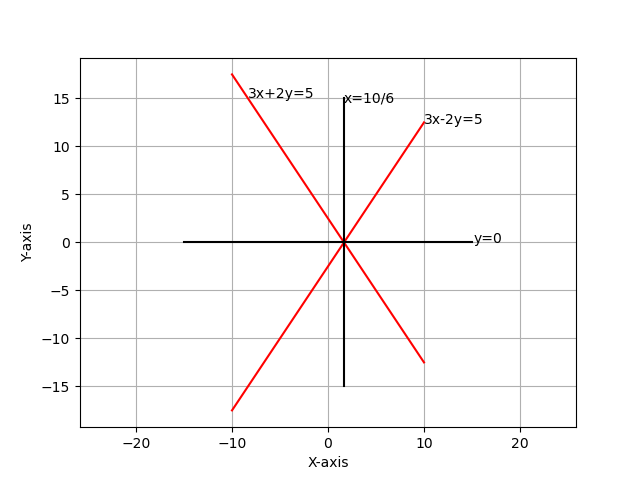
\includegraphics[width=0.7\linewidth]{figs/plot.png}
   \caption{Plot of the given lines and path of the moving point}
   \label{}
\end{figure}
\end{document}  
